% !TeX program = pdflatex
% !TeX encoding = UTF-8
% !TeX spellcheck = en_US
%% Temple University Biology -- dissertation / thesis template (main file)
%% Build:  pdflatex main  ->  bibtex main  ->  pdflatex main  ->  pdflatex main
%%         (or: latexmk -pdf main)
%% Then check the format:  python tools/format_audit.py main.pdf
%%
%% FONT -- choose ONE pair (the Graduate School accepts 12-pt Times New Roman or 10-pt Arial):
%%   Times 12 pt (default):  \documentclass[12pt,oneside,letterpaper]{report}  +  \usepackage{templethesis}
%%   Arial 10 pt:            \documentclass[10pt,oneside,letterpaper]{report}  +  \usepackage[arial]{templethesis}
\documentclass[12pt,oneside,letterpaper]{report}
\usepackage{templethesis}
\usepackage[hidelinks,bookmarksnumbered]{hyperref}   % hidelinks keeps all text black
\usepackage{bookmark}

% ---------------------------------------------------------------- title-page data
% Title: ALL CAPITALS, inverted pyramid (longest line first); no symbols, Greek letters,
% superscripts or formulae -- spell them out (they break keyword searches).
\thesistitle{INSERT THE TITLE OF YOUR DISSERTATION OR THESIS\\HERE IN ALL CAPITAL LETTERS\\AS AN INVERTED PYRAMID}
\thesisauthor{Firstname M. Lastname}   % exactly as on your Temple University transcript
% Doctoral students (default):
\thesistype{Dissertation}
\thesisdegree{DOCTOR OF PHILOSOPHY}
% Master's students -- use these two lines instead (the title page then follows the thesis
% E-Title Page, Handbook Appendix E, including the "Thesis Approvals:" heading):
%   \thesistype{Thesis}
%   \thesisdegree{MASTER OF SCIENCE}
\diplomadate{May 2027}               % official diploma date: December, May or August only
\copyrightyear{2027}
\committee{%
  Advisor Name, Ph.D., Advisory Chair, Department of Biology\\[6pt]
  Member Name, Ph.D., Department of Biology\\[6pt]
  Member Name, Ph.D., Department of Biology\\[6pt]
  Member Name, Ph.D., Department of Biology\\[6pt]
  Member Name, Ph.D., External Member, Department or Institution}

\begin{document}

% ================================================================ FRONT MATTER
% Order required by the Handbook: (Title), Copyright, Abstract, Dedication, Acknowledgments,
% Preface, Table of Contents, Lists.
\pagenumbering{roman}
\maketitlepage                       % page i (number not shown)
\makecopyrightpage                   % page ii (optional; delete this line to omit)
% !TeX root = ../main.tex
\frontsection{ABSTRACT}
% Graduate School rules: the Abstract is TEXT ONLY -- no headings, tables, figures,
% citations, or notes.  It has no word limit, but it should briefly state the problem,
% describe the methods, and summarize the major findings and conclusions.

Replace this paragraph with your abstract. State the problem addressed in the dissertation, describe the research approach and methods, and summarize the major findings and conclusions. The abstract is double-spaced and continues the lower-case Roman page numbering of the front matter.

If you upload movies or other multimedia as supplementary files through ProQuest, the Graduate School requires a description of each file in the Abstract. For example: Supplementary files: Supplementary Movies 1--3 (Chapter 2) show time-lapse recordings of the experiments described in Figure 2.1.

% !TeX root = ../main.tex
% Dedication (optional). The Graduate School template shows no heading on this page;
% \dedication centres the text on the page and lists DEDICATION in the table of contents.
% \\ breaks a line; a blank line starts a new paragraph.  Delete the \input line in
% main.tex to omit this page.
\dedication{%
Replace this text with your dedication.
}
       % optional
% !TeX root = ../main.tex
\frontsection{ACKNOWLEDGMENTS}
% Optional.  Double-spaced; continues the Roman page numbering.

Replace this text with your acknowledgments. Thank your advisor, committee members, collaborators, core facilities, and funding sources here. Grant numbers can be listed in this section or in the acknowledgments of the individual chapters.
  % optional
\tableofcontents
\clearpage
\phantomsection\addcontentsline{toc}{chapter}{LIST OF TABLES}
\listoftables
\clearpage
\phantomsection\addcontentsline{toc}{chapter}{LIST OF FIGURES}
\listoffigures
% !TeX root = ../main.tex
% List of abbreviations (optional; follows the List of Figures and is listed in the
% table of contents).  One \abbrev{short}{long} per line, in alphabetical order.
% Single-spaced within an entry, a blank line between entries.
\frontsection{LIST OF ABBREVIATIONS}
\begin{abbrevlist}
\abbrev{3D}{Three-dimensional}
\abbrev{FRAP}{Fluorescence recovery after photobleaching}
\abbrev{GFP}{Green fluorescent protein}
\abbrev{NPC}{Nuclear pore complex}
\abbrev{PALM}{Photoactivated localization microscopy}
\abbrev{SMLM}{Single-molecule localization microscopy}
\end{abbrevlist}
    % optional LIST OF ABBREVIATIONS

% ================================================================ BODY
\clearpage
\pagenumbering{arabic}               % Chapter 1 begins on page 1
\tocgrouplabel{CHAPTER}
% !TeX root = ../main.tex
% Chapter 1 -- General introduction.  This sample shows the main formatting features:
% numbered headings, citations, a figure, a table, an equation, a block quote and a footnote.
% Replace everything below the \label line with your own text.
\chapter{GENERAL INTRODUCTION}
\label{ch:intro}

\section{Using This Template}

Each chapter lives in its own file in the \texttt{chapters/} folder and is included from \texttt{main.tex}. The chapter heading (``CHAPTER 1'' followed by the title) is centered in capitals at the top of a new page, as the Graduate School requires. Text is double-spaced with a \textonehalf-inch paragraph indent, and every page carries a centered page number inside the 1-inch bottom margin.

Cite references with \verb|\cite{key}|; numbered superscript citations are produced in the order in which sources are first cited\cite{Ma2010three,Balzarotti2017nanometer}. Several sources cited together are sorted and compressed into a range\cite{Betzig2006imaging,Ma2010three,Balzarotti2017nanometer,Lin2019structure}. The reference list at the end of the dissertation is generated by BibTeX from \texttt{references.bib}.

\subsection{Figures}

Figures are numbered by chapter (Figure~\ref{fig:intro:example}). Give every figure a short title in square brackets: that title appears in the List of Figures, while the full legend appears under the figure. Captions are single-spaced and must not use type smaller than 10 points.

\begin{figure}[tbp]
\centering
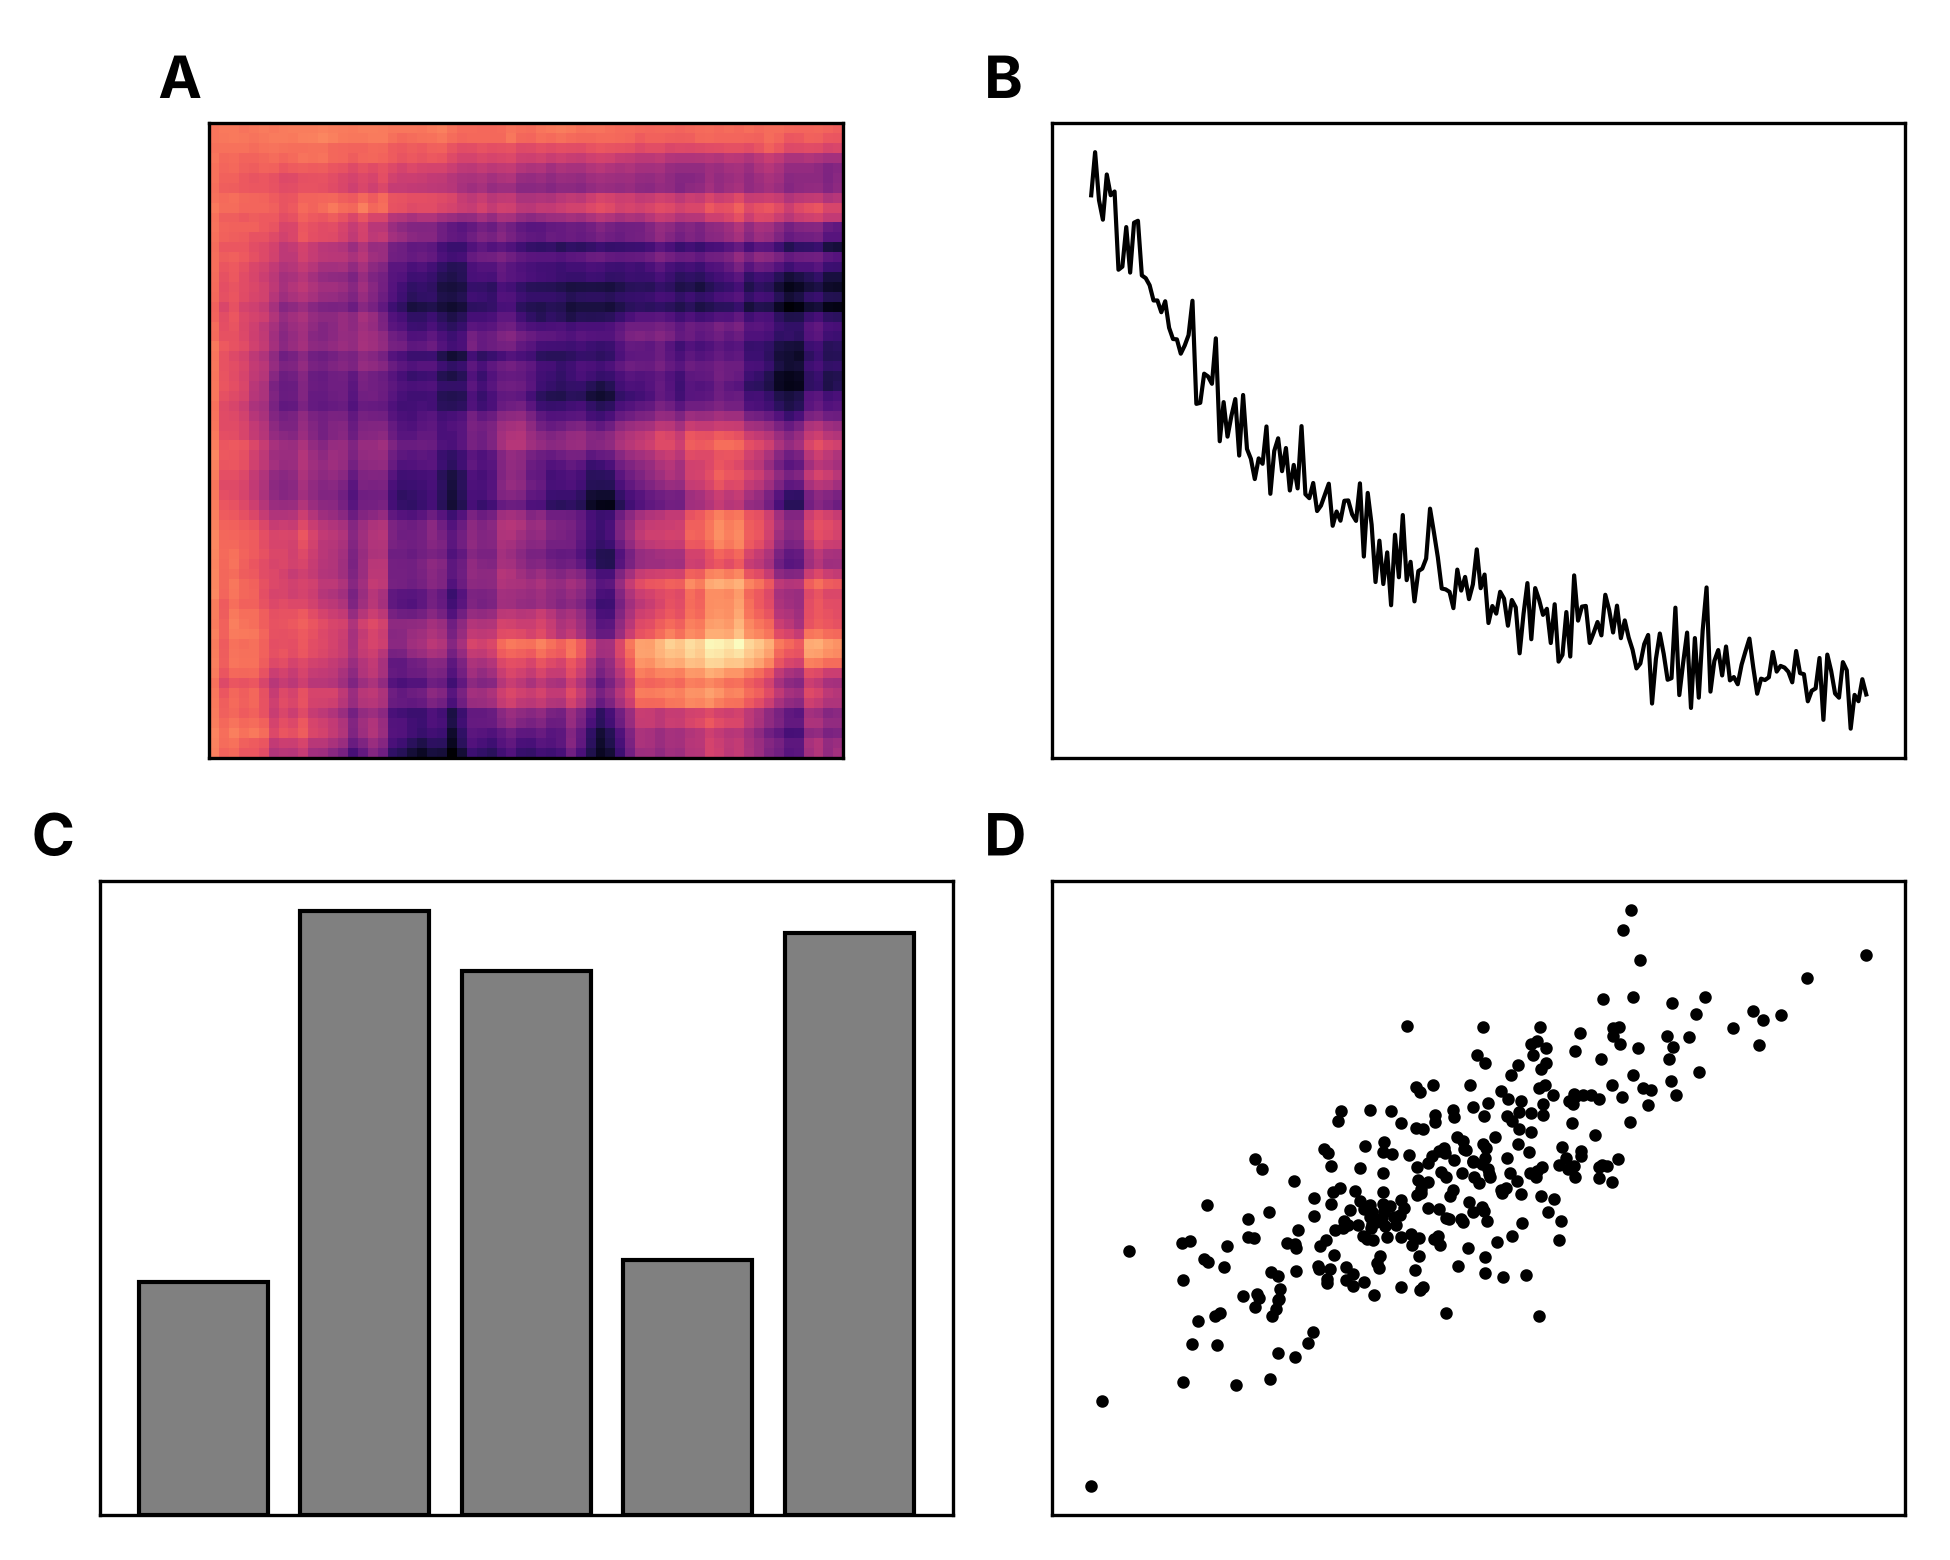
\includegraphics[width=\textwidth,keepaspectratio]{figures/example-figure.png}
\caption[Example of a multi-panel figure]{\textbf{Example of a multi-panel figure.} \textbf{(A)} Panel A description. \textbf{(B)} Panel B description. \textbf{(C)} Panel C description; bars show the mean \textpm{} s.d. of $n = 3$ independent experiments. \textbf{(D)} Panel D description. Scale bar, 1~\textmu m.}
\label{fig:intro:example}
\end{figure}

\subsection{Tables}

Tables are also numbered by chapter (Table~\ref{tab:intro:example}). The \verb|\tablesmall| command reduces the type size of a wide table by one step while keeping it at or above the 10-point minimum.

\begin{table}[tbp]
\centering
\caption[Example of a data table]{\textbf{Example of a data table.} Values are mean \textpm{} s.d.}
\label{tab:intro:example}
\begin{tabular}{@{}lccc@{}}
\toprule
\textbf{Condition} & \textbf{Diffusion coefficient (\textmu m\textsuperscript{2}/s)} & \textbf{Dwell time (ms)} & \textbf{$n$} \\
\midrule
Control   & 0.85 \textpm{} 0.10 & 4.2 \textpm{} 0.6 & 512 \\
Treatment & 0.42 \textpm{} 0.08 & 7.9 \textpm{} 1.1 & 488 \\
\bottomrule
\end{tabular}
\end{table}

\subsection{Equations}

Equations are numbered by chapter, as in Equation~\eqref{eq:intro:msd}:
\begin{equation}
\text{MSD}(t) = \left\langle \left[ r(t_0 + t) - r(t_0) \right]^2 \right\rangle = 2dDt,
\label{eq:intro:msd}
\end{equation}
where $d$ is the number of dimensions and $D$ is the diffusion coefficient.

\section{Other Text Elements}

\subsection{Block Quotations}

Quotations of 40 or more words are set as a block, single-spaced, indented \textonehalf{} inch from both margins, and without quotation marks. The source citation follows the closing punctuation:

\begin{quote}
This is an example of a long quotation of forty words or more. It is set as a free-standing block of text, single-spaced and indented one-half inch from both the left and the right margins, with no surrounding quotation marks, exactly as the Dissertation and Thesis Handbook requires.\cite{Lin2019structure}
\end{quote}

Shorter quotations are integrated into the text and enclosed in quotation marks.

\subsection{Notes}

Most biology dissertations do not need footnotes, but the template formats them as the Handbook requires.\footnote{Footnotes are set in the same type size as the text, single-spaced within a note, with a blank line between notes and the first line indented one-half inch.}

\subsubsection{A third-level heading}

Use at most three heading levels. Only chapters, sections and subsections appear in the Table of Contents; to include third-level headings, change \verb|\setcounter{tocdepth}{2}| to 3 in \texttt{templethesis.sty}.

% !TeX root = ../main.tex
% Chapter 2 -- a research chapter based on a published or submitted manuscript
% ("manuscript-style" chapter).  The chapternote block gives the publication status and
% author contributions.  If the chapter reproduces a published article, check the
% journal's reuse policy and include any permission letter in an appendix, as the
% Dissertation and Thesis Handbook requires.
\chapter{TITLE OF YOUR FIRST RESEARCH CHAPTER IN CAPITAL LETTERS}
\label{ch:manuscript}

\begin{chapternote}
This chapter has been published as: Author, A., Author, B. \& Advisor, C. Title of the article. \textit{Journal Name} \textbf{12}, 345 (2026). Reproduced under the terms of the Creative Commons Attribution 4.0 International License.

Author contributions: C. Advisor designed the experiments. A. Author and B. Author performed the experiments and analyzed the data. A. Author and C. Advisor wrote the manuscript.
\end{chapternote}

\section{Abstract}

A manuscript-style chapter can keep the section structure of the article: Abstract, Introduction, Results, Discussion, and Methods. Replace this text with the chapter abstract.

\section{Introduction}

Replace this text with the introduction of the chapter\cite{Ma2010three}.

\section{Results}

\subsection{First Result Heading}

Replace this text with your results. Supplementary figures can be placed in an appendix and cited as, for example, Figure~\ref{fig:appA:example}.

\subsection{Second Result Heading}

Replace this text with your results.

\section{Discussion}

Replace this text with the discussion.

\section{Methods}

\subsection{Cell Culture}

Replace this text with your methods.

\subsection{Statistical Analysis}

Replace this text with your methods.

% !TeX root = ../main.tex
% Final chapter -- general discussion, conclusions and future directions.
\chapter{GENERAL DISCUSSION AND FUTURE DIRECTIONS}
\label{ch:discussion}

\section{Summary of Findings}

Replace this text with a summary of the main findings of the dissertation, connecting the research chapters (Chapter~\ref{ch:manuscript}) to the questions raised in Chapter~\ref{ch:intro}.

\section{Future Directions}

Replace this text with future directions.

\section{Conclusions}

Replace this text with your conclusions.


% ================================================================ BACK MATTER
\clearpage
\phantomsection
\addcontentsline{toc}{chapter}{REFERENCES}
\bibliographystyle{thesis}           % Nature-style numbered references (see thesis.bst)
\bibliography{references}

\appendix
\tocgrouplabel{APPENDICES}
% !TeX root = ../main.tex
% Appendix A -- supplementary information for a research chapter.  Figures and tables are
% numbered A.1, A.2, ...  The [H] placement keeps supplementary figures in order.
\chapter{SUPPLEMENTARY INFORMATION FOR CHAPTER 2}
\label{app:supplementary}

\begin{chapternote}
This appendix reproduces the Supplementary Information for Chapter~\ref{ch:manuscript}. Supplementary Figure~\textit{N} of the published article corresponds to Figure~A.\textit{N} here.
\end{chapternote}

\section{Supplementary Figures}

\begin{figure}[H]
\centering
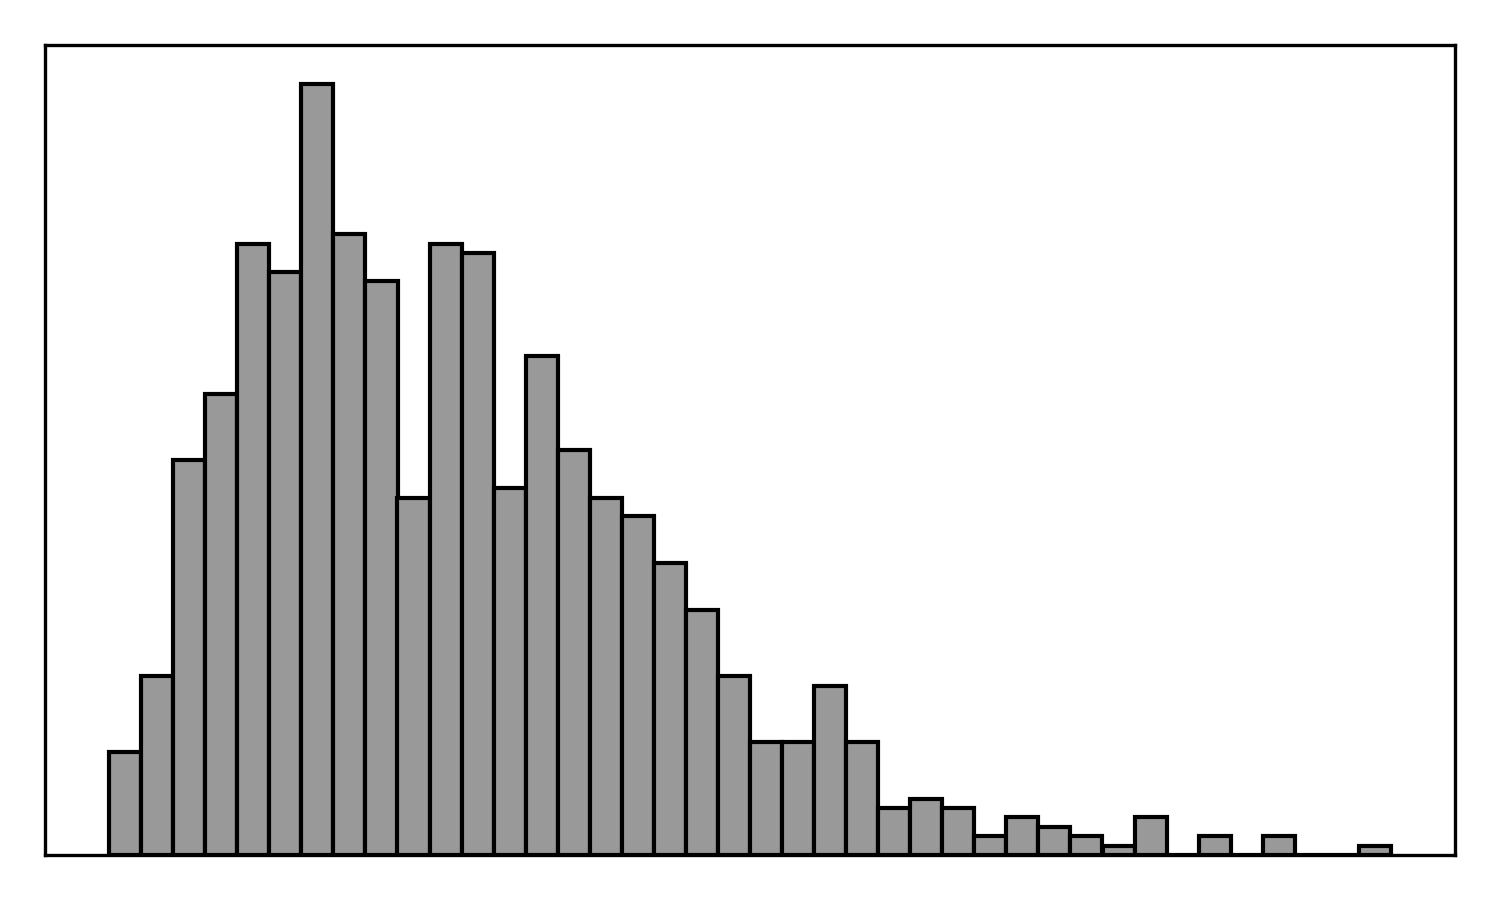
\includegraphics[width=0.8\textwidth,keepaspectratio]{figures/example-supplementary.png}
\caption[Example of a supplementary figure]{\textbf{Example of a supplementary figure.} Replace this legend with the supplementary figure legend.}
\label{fig:appA:example}
\end{figure}

\section{Supplementary Tables}

Wide tables can be set on a landscape page. The page number stays at the bottom of the page in portrait orientation, as the Graduate School requires.

\begin{landscape}
{\singlespacing
\tablesmall\setlength{\tabcolsep}{4pt}
\begin{longtable}{@{}p{1.3in}p{1.3in}p{1.3in}p{1.3in}p{1.3in}p{1.3in}@{}}
\caption[Example of a wide table on a landscape page]{\textbf{Example of a wide table on a landscape page.} Long tables continue across pages, and the header row is repeated.}
\label{tab:appA:wide}\\
\toprule
\textbf{Column 1} & \textbf{Column 2} & \textbf{Column 3} & \textbf{Column 4} & \textbf{Column 5} & \textbf{Column 6}\\
\midrule
\endfirsthead
\multicolumn{6}{@{}l}{\textit{Table \thetable\ (continued)}}\\
\toprule
\textbf{Column 1} & \textbf{Column 2} & \textbf{Column 3} & \textbf{Column 4} & \textbf{Column 5} & \textbf{Column 6}\\
\midrule
\endhead
\bottomrule
\endlastfoot
Row 1 & Value & Value & Value & Value & Value\\
Row 2 & Value & Value & Value & Value & Value\\
Row 3 & Value & Value & Value & Value & Value\\
\end{longtable}}
\end{landscape}


\end{document}
